\chapter{Introduction}
\label{introchap}

The ``Smartwatch Device and App for Continuous Glucose Monitoring'' senior design project\cite{ecesd1814} is sponsored by Biorasis\cite{Biorasis}, located in Storrs, Connecticut. The company goal is to develop a smartwatch-like device that communicates with an implantable, glucose-monitoring device created by the company. The senior design project is a continuation of a project\cite{ecesd1714} completed last year that developed a system and working prototype for a smartwatch-like device as described.

The goals for the senior design team this year are to remove the dependencies imposed by last year's prototype and to create a custom device with a larger screen and added visualization of graphed data. Described in this honors thesis will be the process for developing the new codebase for this system.

\section{Inherited Codebase}

The codebase inherited from last year's project is heavily based on the TinyScreen SmartWatch Tutorial by TinyCircuits\cite{tinywatchtut}, but uses the Tinyscreen+\cite{tinyplus} for the microcontroller and display. The firmware is written in Arduino, a simple platform for writing C++ code for embedded devices. The inherited project includes 41 files inside a single directory. Of these files, 14 files involve C++ code for a Kalman filter and were autogenerated from MATLAB, 24 files are C++ code files from an Arduino Bluetooth library included with the TinyScreen SmartWatch Tutorial, 2 files are C++ files defining a custom frequency analysis function, and the last file is the .ino Arduino source file for the project. These files and their relationships are graphed in \figref{fig:inherited_organization}. It is made clear from the depicted dependency graph that 17 of the files have no impact on the smartwatch firmware and can be safely removed. Of the remaining 24 files, 23 come from the external Bluetooth library. This means that the remaining .ino file represents the majority of the firmware code.

\begin{figure}[htbp]
    \caption[Organization of Inherited Codebase]{
    A graph of the dependencies within the inherited codebase shows that 17 files are completely separated from the main Arduino source file, Float\_Smart\_Watch\_ARM.ino. As a result, these files may be removed from the project without consequence.
    }
    \begin{center}
    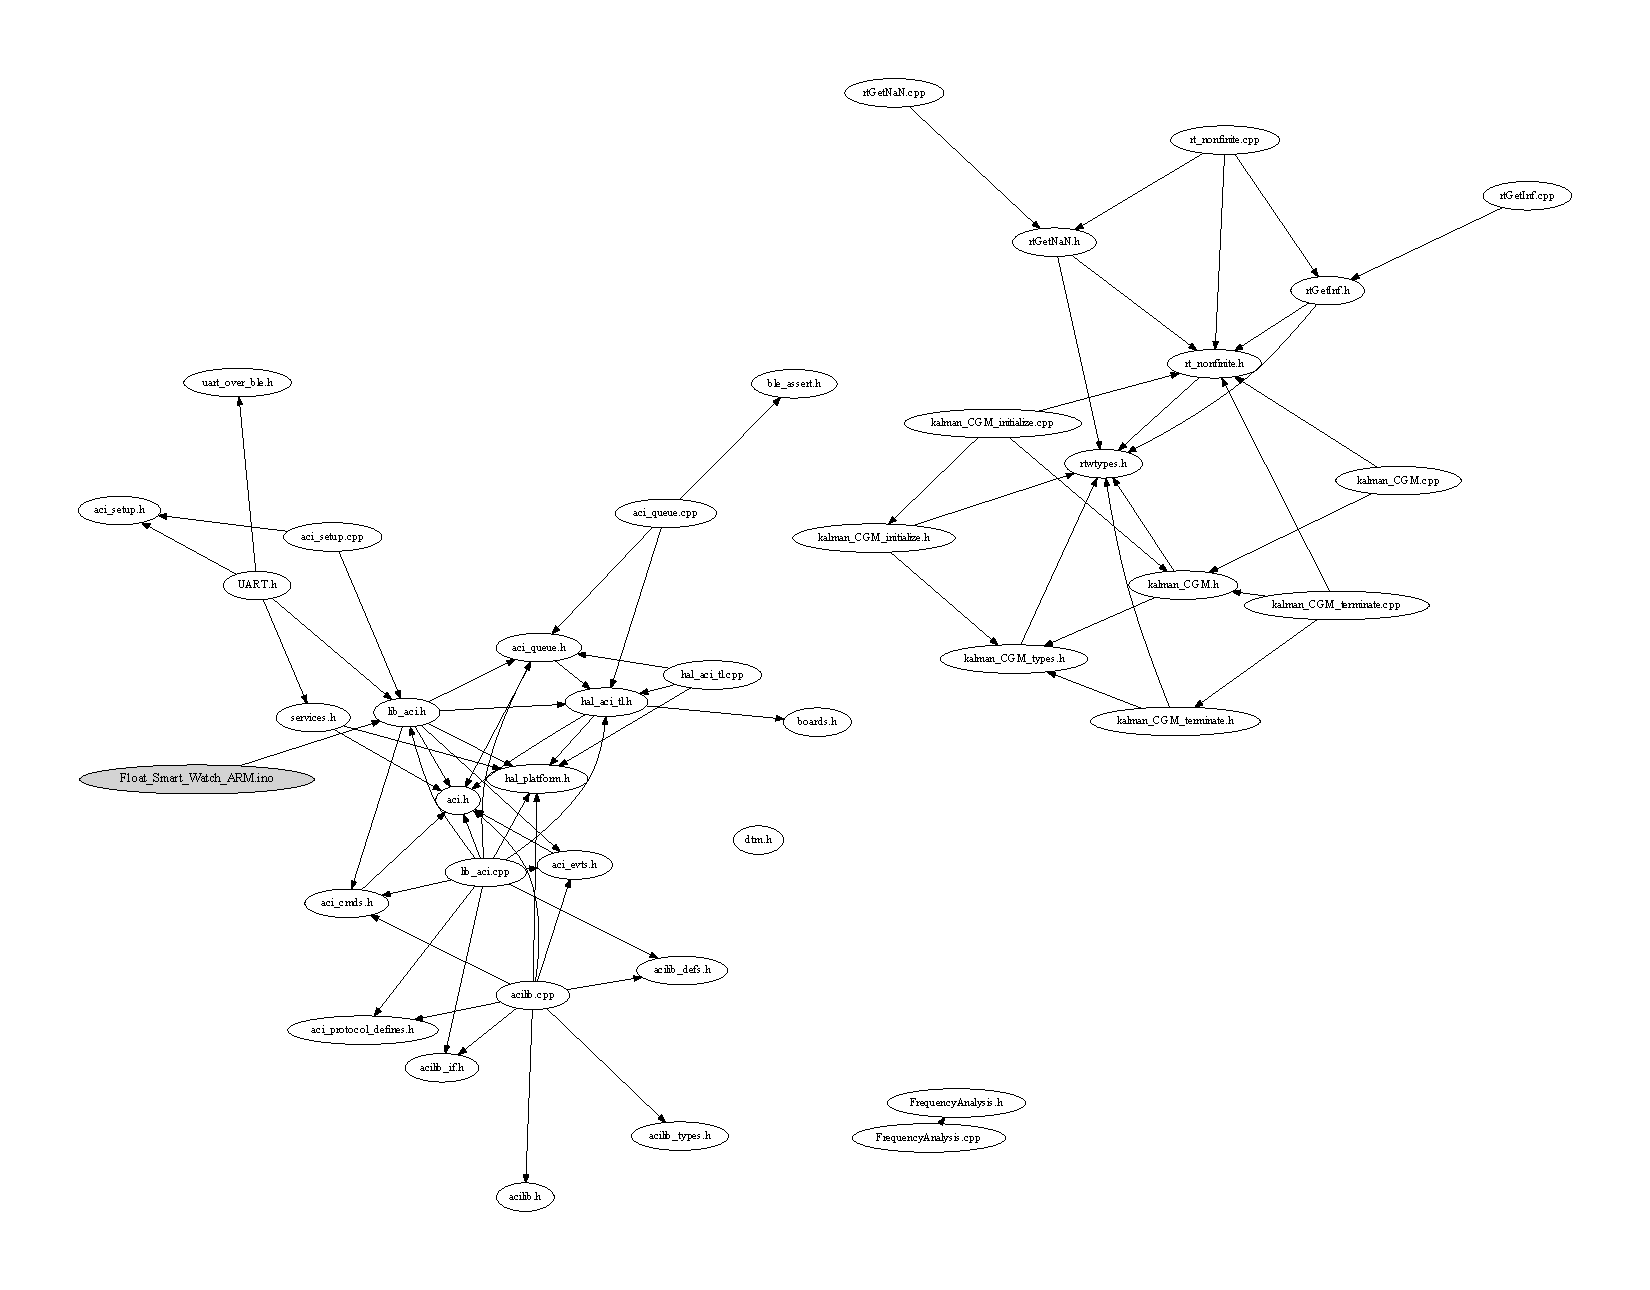
\includegraphics[width=\textwidth,keepaspectratio]{figs/inherited_organization.pdf}
    \end{center}
\label{fig:inherited_organization}
\end{figure}

Having the majority of the firmware localized to a single file creates non-modular code\footnote{In computer science, there is a concept called ``separation of concerns'' that says a computer program should be separated into distinct sections that each handle smaller portions of the code. Such a well-organized program is called a modular program\cite{wikiSoC}.}. The logical sections of this file should be determined and used to create distinct program files that would increase organization and readability of the codebase. The logical sections of this file are determined to be as follows:

\singlespacing
\begin{itemize}
  \item{} Code related to reading the current battery level.
  \item{} Code related to handling Bluetooth messages and the Bluetooth library.
  \item{} Code related to handling external button presses.
  \item{} Code related to managing the current time and timers.
  \item{} Code related to writing to the display.
  \item{} Code related to taking a measurement from the implantable biosensor.
  \item{} Code responsible for interconnecting the above into a single project.
\end{itemize}
\doublespacing
The new codebase will implement these logical sections in order to rewrite the firmware of the smartwatch in a more modular fashion.

\section{Atmel Advanced Software Framework}
The dependency on the Tinyscreen+ board and associated Arduino platform needs to be removed from the inherited smartwatch design, to give the sponsor company more control over the hardware of their product and produce devices at a cheaper price. In replacement of Arduino, the Atmel Advanced Software Framework (ASF)\cite{ASF} is used as a platform for the new codebase. The decision to use ASF libraries rather than the Arduino platform comes partially from the fact that Arduino hides a majority of control from the programmer. For instance, in an Arduino project on a Windows machine, all of the header files that directly control the embedded device are located in the AppData folder, which is hidden from the user and not accessible by normal means. In contrast, a project created using ASF libraries would place all related header files into subdirectories that can be easily located from the project directory. A decision to use ASF thus results in a more complete and localized codebase. Additionally, Arduino is written in C++, whereas the C programming language used by ASF libraries is better suited for embedded applications\footnote{This claim is made by personal preference.}.

The Atmel Advanced Software Framework offers easier control of a target microcontroller (MCU\footnote{Microcontroller unit.}) by providing an abstraction to the MCU hardware. In order to reduce the size of the codebase, certain hardware abstractions can be enabled or disabled through ASF. For simplicity, the MCU used in the new codebase is the same as the MCU used in the inherited codebase: the ATSAMD21G18A\cite{samd21}. The following components of this MCU are made available through ASF to the codebase:

\singlespacing
\begin{itemize}
  \item{} Sleep manager (service)
  \item{} Delay routines (service) [systick]
  \item{} ADC - Analog-to-Digital Converter (driver) [callback]
  \item{} EVSYS - Event System (driver) [polled]
  \item{} EXTINT - External Interrupt (driver) [callback]
  \item{} PORT - GPIO Pin Control (driver)
  \item{} RTC - Real Time Counter Driver (driver) [calendar\_callback]
  \item{} SERCOM SPI - Serial Peripheral Interface (driver) [callback]
  \item{} SYSTEM - Core System Driver (driver)
  \item{} TC - Timer Counter (driver) [callback]
  \item{} TCC - Timer Counter for Control Applications (driver) [callback]
\end{itemize}
\doublespacing
In order to increase parallelism in the smartwatch, the majority of the MCU hardware components use callbacks, which are called in response to hardware interrupts.

\section{Smartphone Application}
A smartphone app is also provided by last year's project, which is written in Android Studio and is modified from the Android application included with the TinyScreen SmartWatch Tutorial. The smartphone app is not heavily modified from last year's version for the new codebase. The only improvements made to it are additions to the permissions and setup of the application, in order to allow it to run on more modern android devices\footnote{The inherited Android application was based on Android application code from 2014, and desperately needed updating for support in modern phones.}.

The basic functions of the smartphone app include displaying the glucose measurements received from the smartwatch, sending notifications to the smartwatch, and sending commands to the smartwatch that set the current time and measurement period. The smartphone app stores received data in a .csv file that it creates within the phone memory. The smartphone app requests from the Android phone that it has permission to discover and pair with Bluetooth devices, connect to paired Bluetooth devices, write to an external storage, access the approximate location of the smartphone, and bind to a notification listener service. The minimum Android version configured for the smartphone app is Android Jelly Bean 4.3.x, API level 18. The target Android version configured for the smartphone app is Android Nougat 7.1, API level 25.
